\documentclass[notheorems,10pt]{beamer}

% pdflatex
% \usepackage[utf8]{inputenc}
% \usepackage[T1]{fontenc}
% \usepackage[czech]{babel}
% \usepackage{lmodern}

% lualatex
\usepackage{fontspec}
\usepackage{polyglossia}
\usepackage{lmodern}

% math
\usepackage{amsmath}
\usepackage{amsthm}
\usepackage{amssymb}
\usepackage{tikz}
\usetikzlibrary{%
	shapes.geometric,calc,arrows,decorations.markings,decorations.pathmorphing,spy
}
\usepackage{pgfplots}
% \pgfplotsset{compat=1.18}
\usepackage{ifthen}
\usepackage{bbding}								% fancy tick/cross symbol
\usepackage{booktabs}							% fancy tables
\usepackage{datatool}
\usepackage{nicefrac}
\usepackage{fontawesome}
\usepackage{appendixnumberbeamer}
% \usepackage{todonotes}
\usepackage{minted}

\usepackage{graphicx}
\usepackage{listings}
\usepackage{svg}

\lstset{
    basicstyle=\ttfamily\small,
    keywordstyle=\color{blue}\bfseries,
    commentstyle=\color{gray},
    frame=single,
    breaklines=true,
    escapeinside={(*}{*)},
}

% unicode characters
\hypersetup{%
	unicode=true,
	pdfstartview=Fit,
	pdfview=Fit,
	pdfpagemode=UseNone
}

%% Czech-style trigonometric functions
\DeclareMathOperator{\tg}{\mathrm{tg}}
\DeclareMathOperator{\arctg}{\mathrm{arctg}}
\DeclareMathOperator{\arccotg}{\mathrm{arccotg}}
\DeclareMathOperator{\cotg}{\mathrm{cotg}}

%% Other Czech stuff
\newcommand{\uv}[1]{,,#1``}

%% Other custom commands
\DeclareMathOperator{\sgn}{\mathrm{sgn}}
\DeclareMathOperator{\graf}{\mathrm{graf}}
\newcommand{\ceq}{\mathrel{\mathop:}=}
\newcommand{\veps}{\varepsilon}
\newcommand{\dx}{\mathrm{d}x}
\newcommand{\dy}{\mathrm{d}y}
\newcommand{\dz}{\mathrm{d}z}
\newcommand{\dt}{\mathrm{d}t}
\renewcommand{\Re}{\mathrm{Re}\,}
\renewcommand{\Im}{\mathrm{Im}\,}

%% zvyrazneni
\renewcommand{\emph}[1]{\textit{#1}}
\newcommand{\notion}[1]{\textbf{#1}}
\newcommand{\eng}[1]{\textit{#1}}
\newcommand{\tred}[1]{{\color{red}#1}}
\newcommand{\tblue}[1]{{\color{blue}#1}}
\newcommand{\tbrown}[1]{{\color{brown}#1}}
\newcommand{\tgray}[1]{{\color{gray}#1}}
\newcommand{\tgreen}[1]{{\color{green!60!black}#1}}

%% nice link
\newcommand{\nicelink}[2]{\href{#1}{{\small\faicon{external-link}}\,#2}}
\newcommand{\courses}[1]{\href{https://courses.fit.cvut.cz/#1}{{\small\faicon{external-link}}\,#1}}

%% special symbols
\newcommand{\NN}{\mathbb{N}}
\newcommand{\ZZ}{\mathbb{Z}}
\newcommand{\QQ}{\mathbb{Q}}
\newcommand{\RR}{\mathbb{R}}
\newcommand{\eRR}{\overline{\mathbb{R}}}
\newcommand{\pinfty}{+\infty}
\newcommand{\minfty}{-\infty}
\newcommand{\bigO}{\mathcal{O}}
\newcommand{\bigOmg}{\Omega}
\newcommand{\bigomg}{\omega}
\newcommand{\bigth}{\Theta}
\newcommand{\bigo}{o}
\newcommand{\ee}{\mathrm{e}}
\newcommand{\diag}{\mathrm{diag}}

%% vectors
\newcommand{\vx}{\mathbf{x}}
\newcommand{\vy}{\mathbf{y}}
\newcommand{\vz}{\mathbf{z}}
\newcommand{\va}{\mathbf{a}}
\newcommand{\vb}{\mathbf{b}}
\newcommand{\vc}{\mathbf{c}}
\newcommand{\ve}{\mathbf{e}}
\newcommand{\vs}{\mathbf{s}}

%% matrices
\newcommand{\mA}{\mathbf{A}}
\newcommand{\mB}{\mathbf{B}}
\newcommand{\mC}{\mathbf{C}}
\newcommand{\mD}{\mathbf{D}}
\newcommand{\mE}{\mathbf{E}}
\newcommand{\mM}{\mathbf{M}}
\newcommand{\mP}{\mathbf{P}}

%% mutlivariate
\newcommand{\grad}{\mathrm{grad}}
\DeclareMathOperator*{\cart}{\scalebox{2}{\times}}

%% TikZ global styles
\tikzset{%
	thickaxis/.style={thick,->}
}

%% Vzhled beamer prezentace
\useoutertheme{infolines}
\useinnertheme[shadow]{rounded}
\usecolortheme{rose}
\usefonttheme{professionalfonts}

\setbeamertemplate{theorems}[ams style]

%% logo
\pgfdeclareimage[height=.7cm]{logo}{attachments/ctu_logo.pdf}
\logo{\pgfuseimage{logo}}

%% Titulni stranka
\title[HiRoPE]{HiRoPE: Length Extrapolation for Code Models Using Hierarchical Position}
\author[Maksim Sapronov]{%
    Authors: Kechi Zhang, Ge Li, Huangzhao Zhang, Zhi Jin \\
    \bigskip
    Maksim Sapronov
}
\institute[FIT CTU]{%
        Knowledge Engineering Seminar \\
        Faculty of Information Technology \\
        Czech Technical University in Prague
}
\date{}

\newtheoremstyle{presentation}%
	{0pt}% space above
	{0pt}% space below
	{\normalfont}% body font
	{}% indent amount
	{\bfseries}% theorem head font
	{:}% punctuation after theorem head
	{.5em}% space after theorem head
	{}% head spec (?)

\theoremstyle{presentation}
\newtheorem*{defi}{Definition}

\setbeamerfont*{block title example}{series=\bfseries,size=\normalsize,family=\sffamily,shape=\upshape}
\setbeamerfont*{block title}{series=\bfseries,size=\normalsize,family=\sffamily,shape=\upshape}

\makeatletter
\def\th@tweek{%
	\normalfont
	\def\inserttheoremblockenv{exampleblock}
}
\theoremstyle{tweek}
\newtheorem*{prik}{Příklad}
\makeatother

%% dalsi vylepseni
\setbeamertemplate{frametitle continuation}[from second][(pokračování)]
\setbeamertemplate{navigation symbols}{}
\usefonttheme[onlymath]{serif}
\setbeamertemplate{sections/subsections in toc}[square]

%% other
\setbeamertemplate{blocks}[rounded][shadow=true]
\setbeamertemplate{headline}{%
	\begin{beamercolorbox}{section in head/foot}
		\vskip2pt\insertnavigation{\paperwidth}\vskip2pt
	\end{beamercolorbox}
}
\setbeamertemplate{frametitle}{%
	\nointerlineskip
	\begin{beamercolorbox}[ht=1.6em,wd=\paperwidth,sep=0.2cm]{frametitle}
	\vbox{}\vskip-2ex%
	\strut\insertframetitle\strut
	\vskip-0.8ex%
	\end{beamercolorbox}
}



\def\mySectionBg{%
  \begin{tikzpicture}
    \useasboundingbox (current page.north west) rectangle (current page.south east);
    \begin{scope}
      \clip (0,0) rectangle (\paperwidth,\paperheight);
      \node at (0.75\paperwidth,0.25\paperheight) {\color{blue!20}$\displaystyle\int_a^b f(x) \dx = \lim_{n\to\infty} \mathcal{J}(\sigma_n, f, a, b)$};
    \end{scope}
  \end{tikzpicture}
}

\def\q{{\mathbf q}}
\def\k{{\mathbf k}}
\def\v{{\mathbf v}}
\def\p{{\mathbf p}}
\def\x{{\mathbf x}}
\def\m{{\mathbf m}}
\def\W{{\mathbf W}}
\def\R{{\mathbf R}}
\def\Q{{\mathbf Q}}
\def\K{{\mathbf K}}
\def\V{{\mathbf V}}
\def\L{{\cal L}}

\begin{document}

\begin{frame}
  \titlepage
\end{frame}

%%
%% Motivation
%%
\section[Motivation]{Motivation}

% Inductive bias: Main idea
\begin{frame}
	\frametitle{Inductive bias: Main idea}

        \pause
	\begin{defi}
		\notion{Inductive bias} is prior knowledge about the nature of the data that is somehow incorporated into a machine learning model.
        \end{defi}
        \begin{center}
            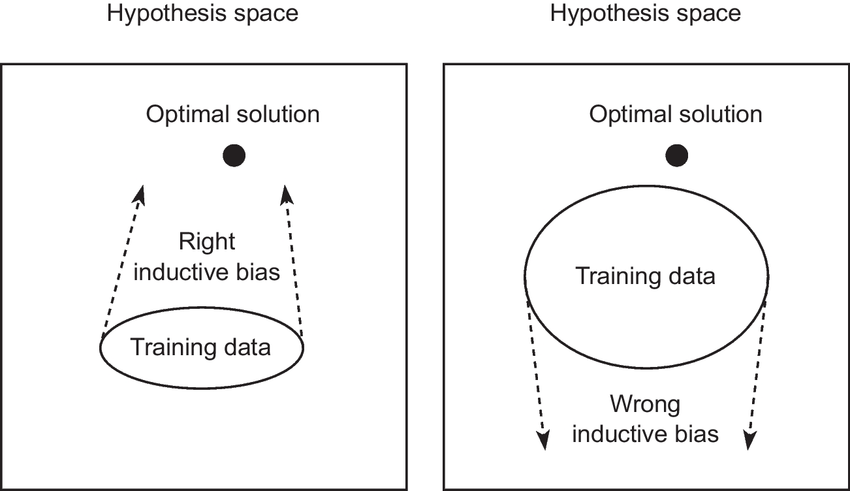
\includegraphics[height=0.5\textheight]{attachments/ind_bias.png}
        \end{center}
        
        \pause
	Code in comparison with natural language has a huge number of constraints  \\
        that could lead the model to a better convergence point.
\end{frame}

% Inductive bias: Hierarchical code structure
\begin{frame}[fragile]
	\frametitle{Inductive bias: Hierarchical code structure}

        \begin{columns}
        \column{0.05\textwidth}

        \column{0.5\textwidth}
        \begin{center}
            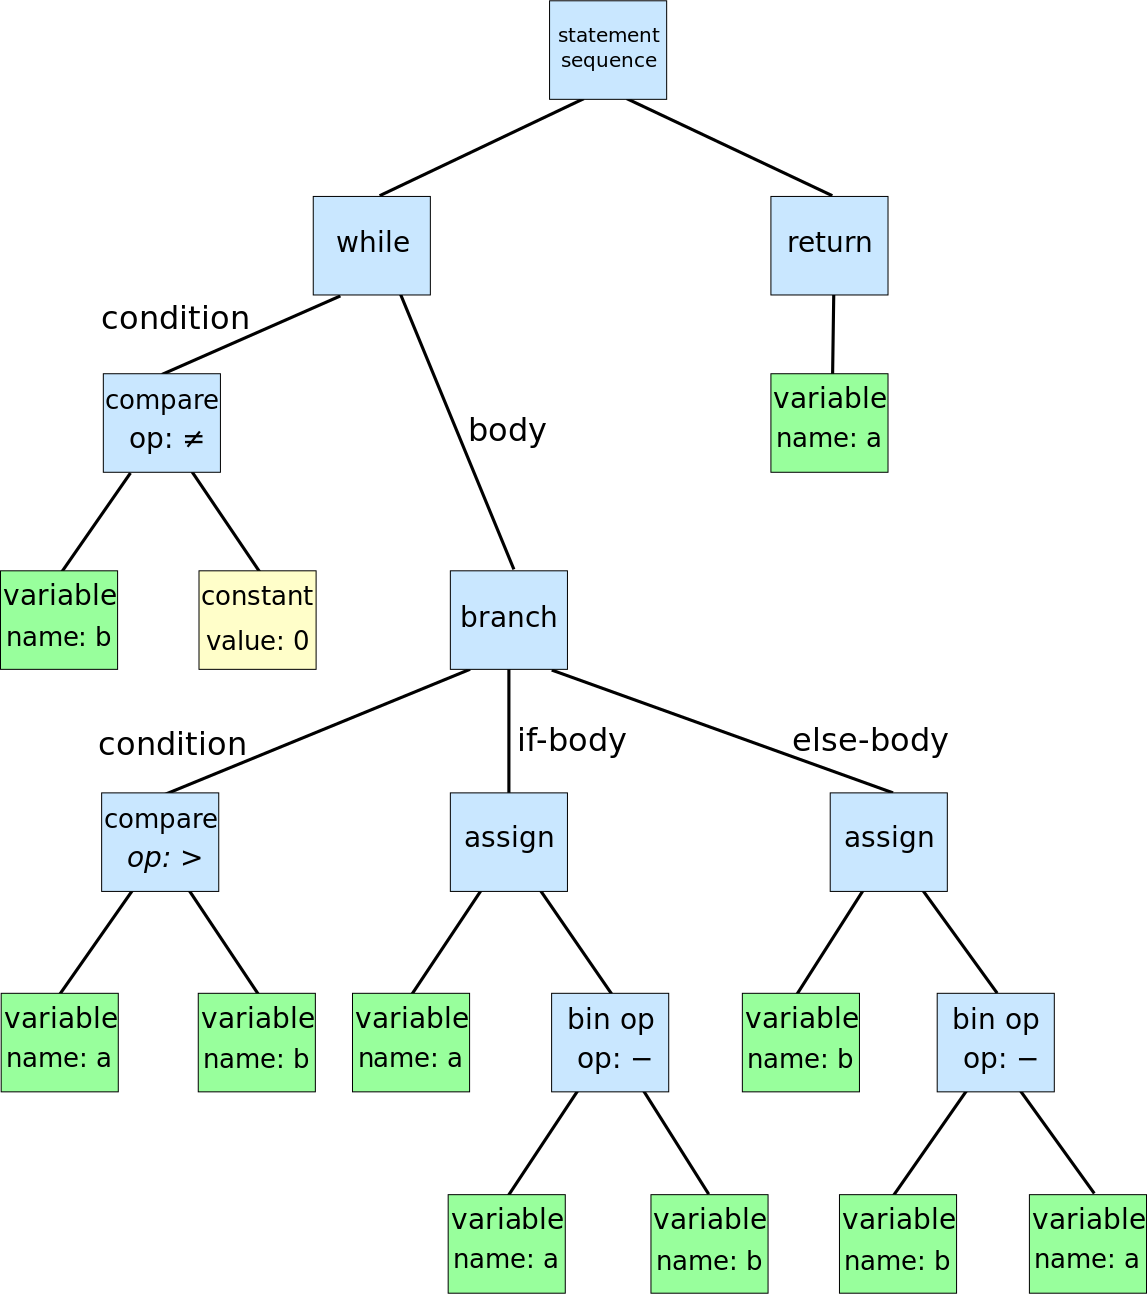
\includegraphics[height=0.7\textheight]{attachments/AST.png}
        \end{center}
        
        \column{0.4\textwidth}
        \begin{lstlisting}[language=Python]
while b != 0:
    if a > b:
        a = a - b
    else:
        b = b - a
return a
        \end{lstlisting}
        \column{0.05\textwidth}
        \end{columns}

    \vfill
    \vfill
    {\centering
    \textit{Abstract syntax tree for the Euclidean algorithm.}
    \par}
\end{frame}

% Long contexts
\begin{frame}
	\frametitle{Long contexts}

        \begin{itemize}
            \item Code modeling task requires the context of the entire project to be included, resulting in a large context window size.
            \vfill
            \item LLMs are typically pre-trained with a context length ranging from 2k to 16k tokens and use RoPE, which has terrible extrapolation ability.
            \vfill
            \item Methods for redefining positional encoding without model fine-tuning stage are in demand nowadays.
        \end{itemize}

        \begin{columns}
        \column{0.5\textwidth}
        \begin{center}
            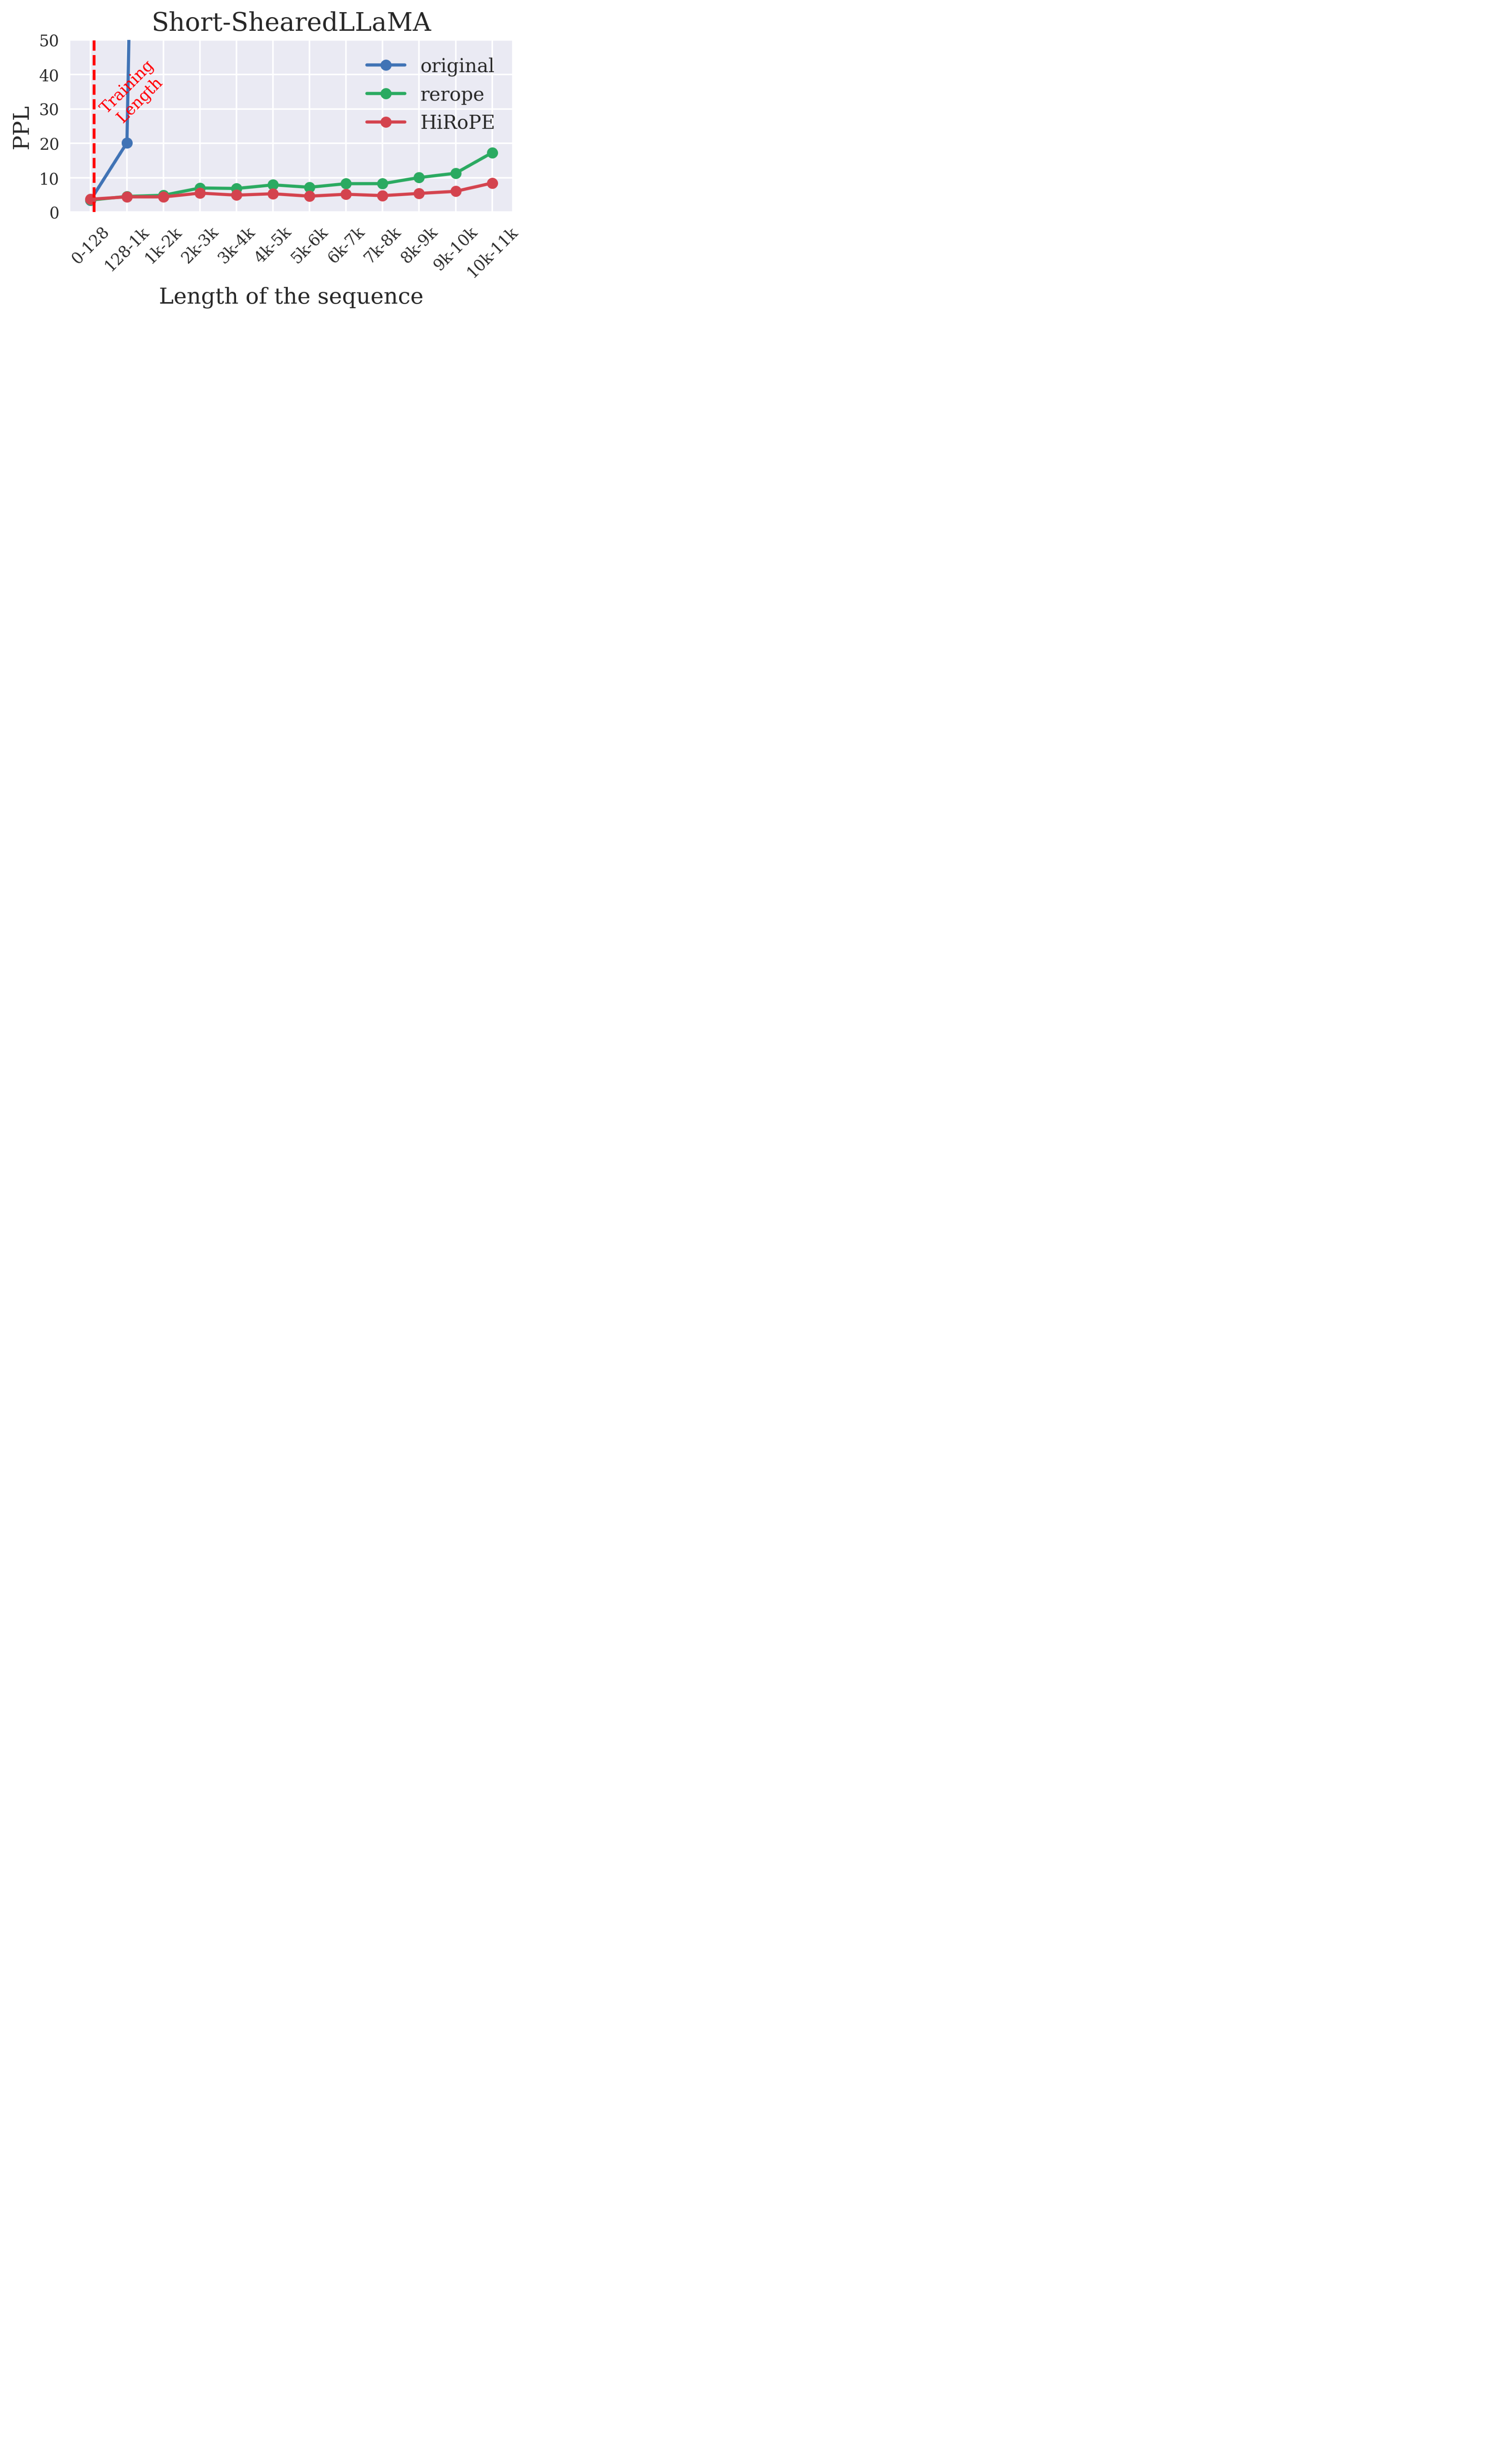
\includegraphics[width=0.9\textwidth]{attachments/extrapolation_1.pdf}
        \end{center}
        \column{0.5\textwidth}
        \begin{center}
            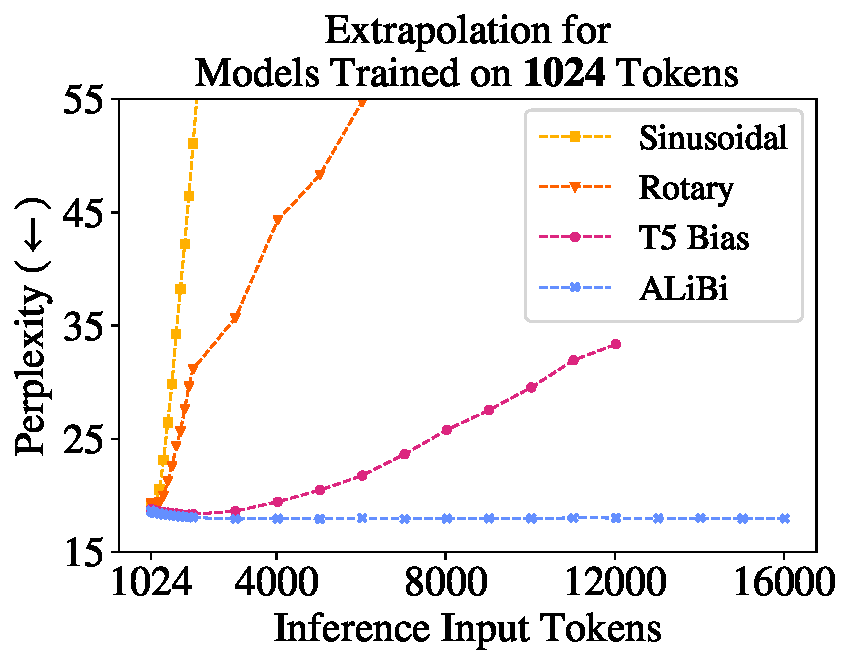
\includegraphics[width=0.9\textwidth]{attachments/extrapolation_2.pdf}
        \end{center}
        \end{columns}
        
\end{frame}

%%
%% Preliminary
%%
\section[Preliminary]{Preliminary}

% A quick overview of the Transformer architecture
\begin{frame}
    \frametitle{A quick overview of the Transformer architecture}
    
    \begin{center}
        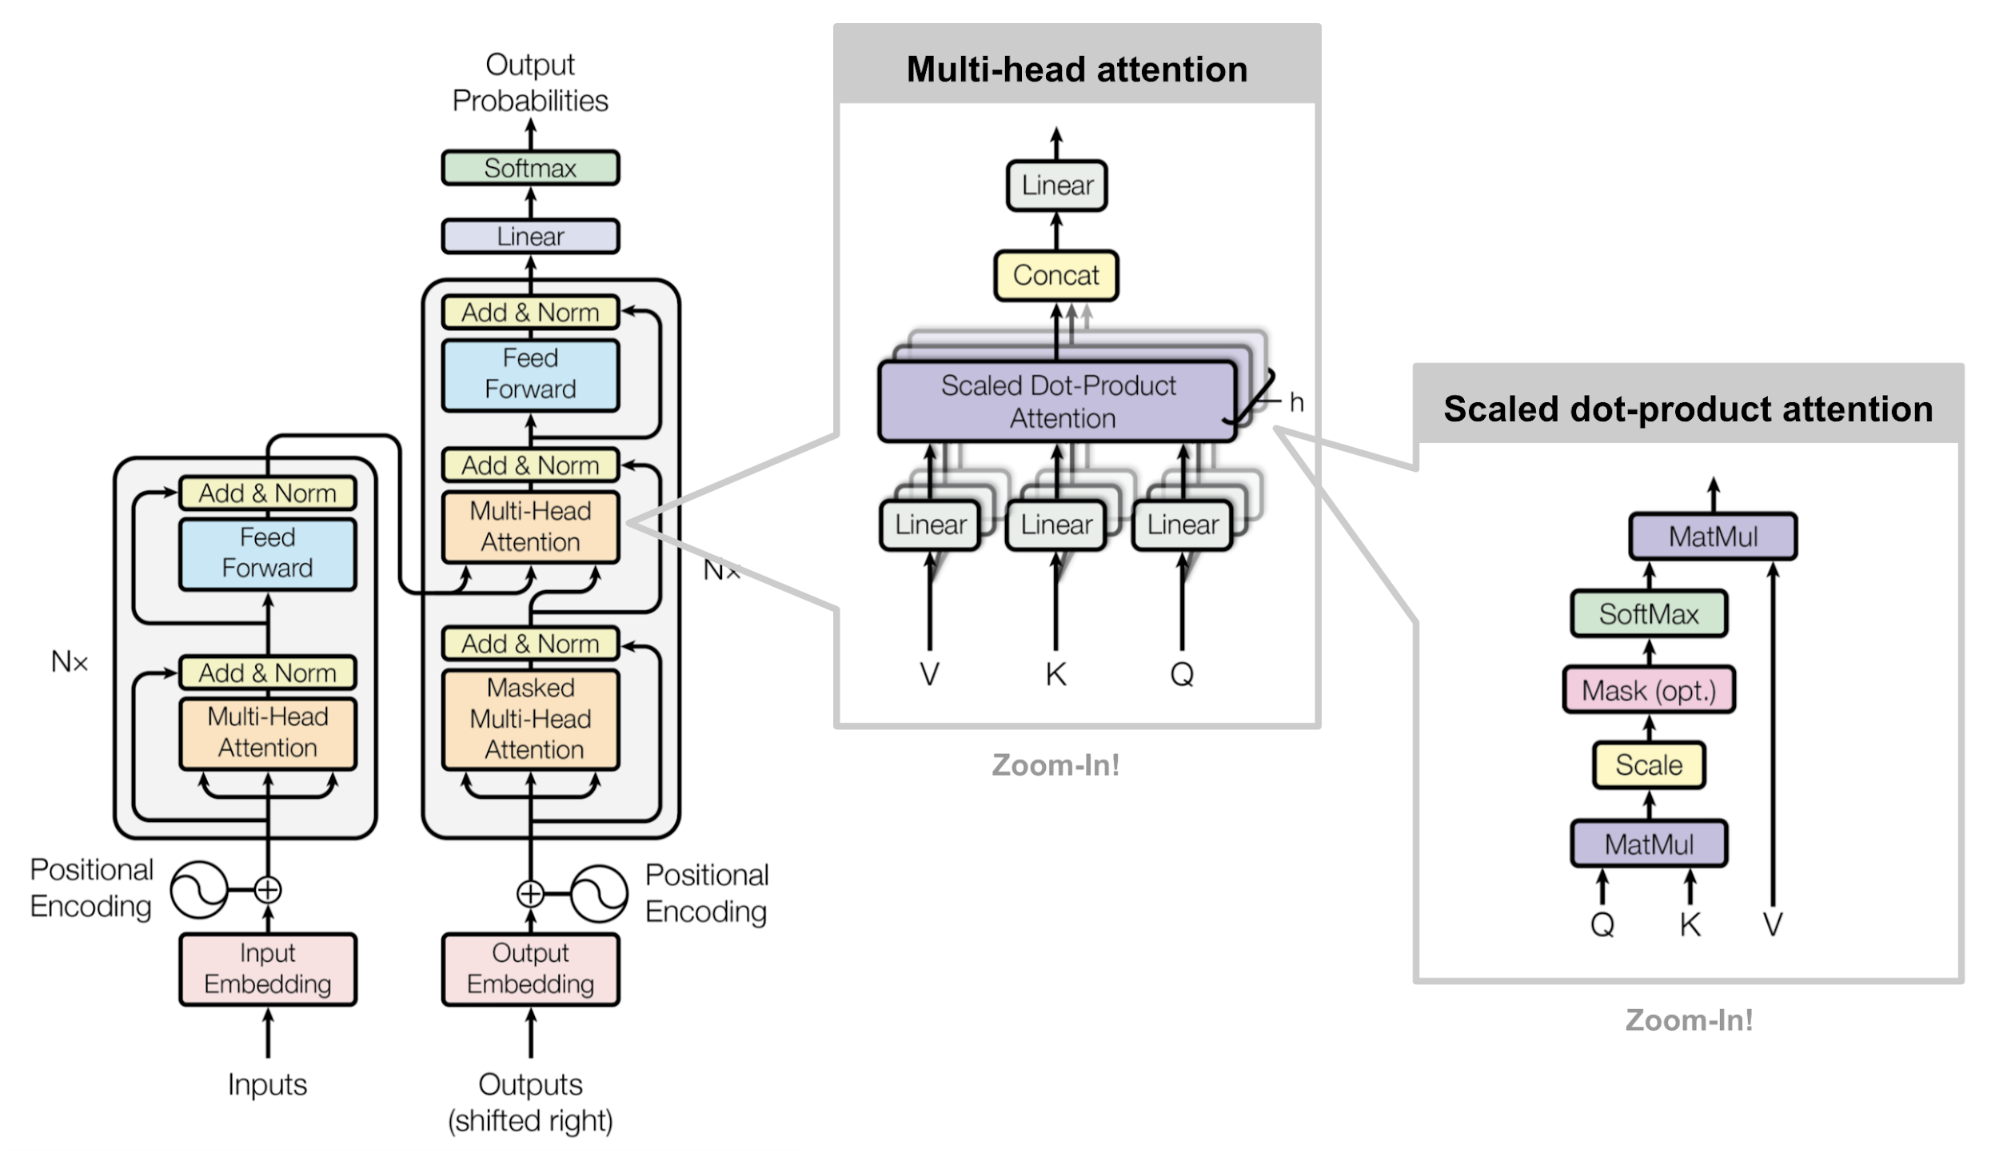
\includegraphics[width=0.9\textwidth]{attachments/transformer.png}
        \\[1ex]
        \textit{The full model architecture of the original transformer.}
    \end{center}
\end{frame}

% Attention mechanism: Notations
\begin{frame}
    \frametitle{Attention mechanism: Notations}

    \pause
    Let $\x_j\in \mathbb{R}^{d}$ be a $d$-dimensional word embedding vector of the $j^{th}$ token without position information. Queries, keys, and value representations are denoted as follows:
    \begin{equation*}
	\begin{aligned}
		\q_m &=f_q(\x_m, m),\\
		\k_n &=f_k(\x_n, n),\\
		\v_n &=f_v(\x_n, n),\\
	\end{aligned}
    \end{equation*}
    where $\q_m,\k_n$ and $ \v_n$ incorporate the $m^{th}$ and $n^{th}$ positions through $f_q,f_k$ and $f_v$, respectively.
    \vfill
    Then the rest part of the attention is
    \begin{equation*}
        a_{m,n} = \frac{\exp\left(\frac{\q_m^{\intercal}\k_n}{\sqrt{d}}\right)}{\sum_{j=1}^{N}\exp\left(\frac{\q_m^{\intercal}\k_j}{\sqrt{d}}\right)},
        \qquad
        \mathbf{o}_m = \sum_{n=1}^{N}a_{m,n}\v_{n}.
    \end{equation*}
\end{frame}

% Positional encoding baselines
\begin{frame}
    \frametitle{Positional encoding baselines}

    \textbf{No Positional Encoding (NoPE)}
    \begin{equation*}
        f_{t:t\in\{q,k,v\}}(\x_m,m):=\W_{t:t\in\{q,k,v\}}\x_m
    \end{equation*}

    \pause
    \vfill
    
    \textbf{Absolute Position Embedding}
    \begin{equation*}
        f_{t:t\in\{q,k,v\}}(\x_m, m) :=
        \begin{cases} 
            \W_{t:t\in\{q,k,v\}}(\x_m + \p_m), & \text{if it is the first transformer layer}, \\[0.4cm]
            \W_{t:t\in\{q,k,v\}}\x_m, & \text{otherwise},
        \end{cases}
    \end{equation*}
    where $\p_m\in\mathbb{R}^{d}$ is a $d$-dimensional vector depending of the position of token $\x_m$. It can be learned directly or expressed with sinusoidal function
    
    \begin{equation*}
	\begin{cases}
		\p_{m,2t}&=\sin(m/10000^{2t/d})\\
		\p_{m,2t+1}&=\cos(m/10000^{2t/d})
	\end{cases},
    \end{equation*}
    in which $\p_{m,2t}$ is the $2t^{th}$ element of $\p_m$.
\end{frame}


%%
%% RoPE
%%
\section[RoPE]{RoPE}

% RoPE: General idea
\begin{frame}
    \frametitle{RoPE: General idea}
    
    \begin{center}
        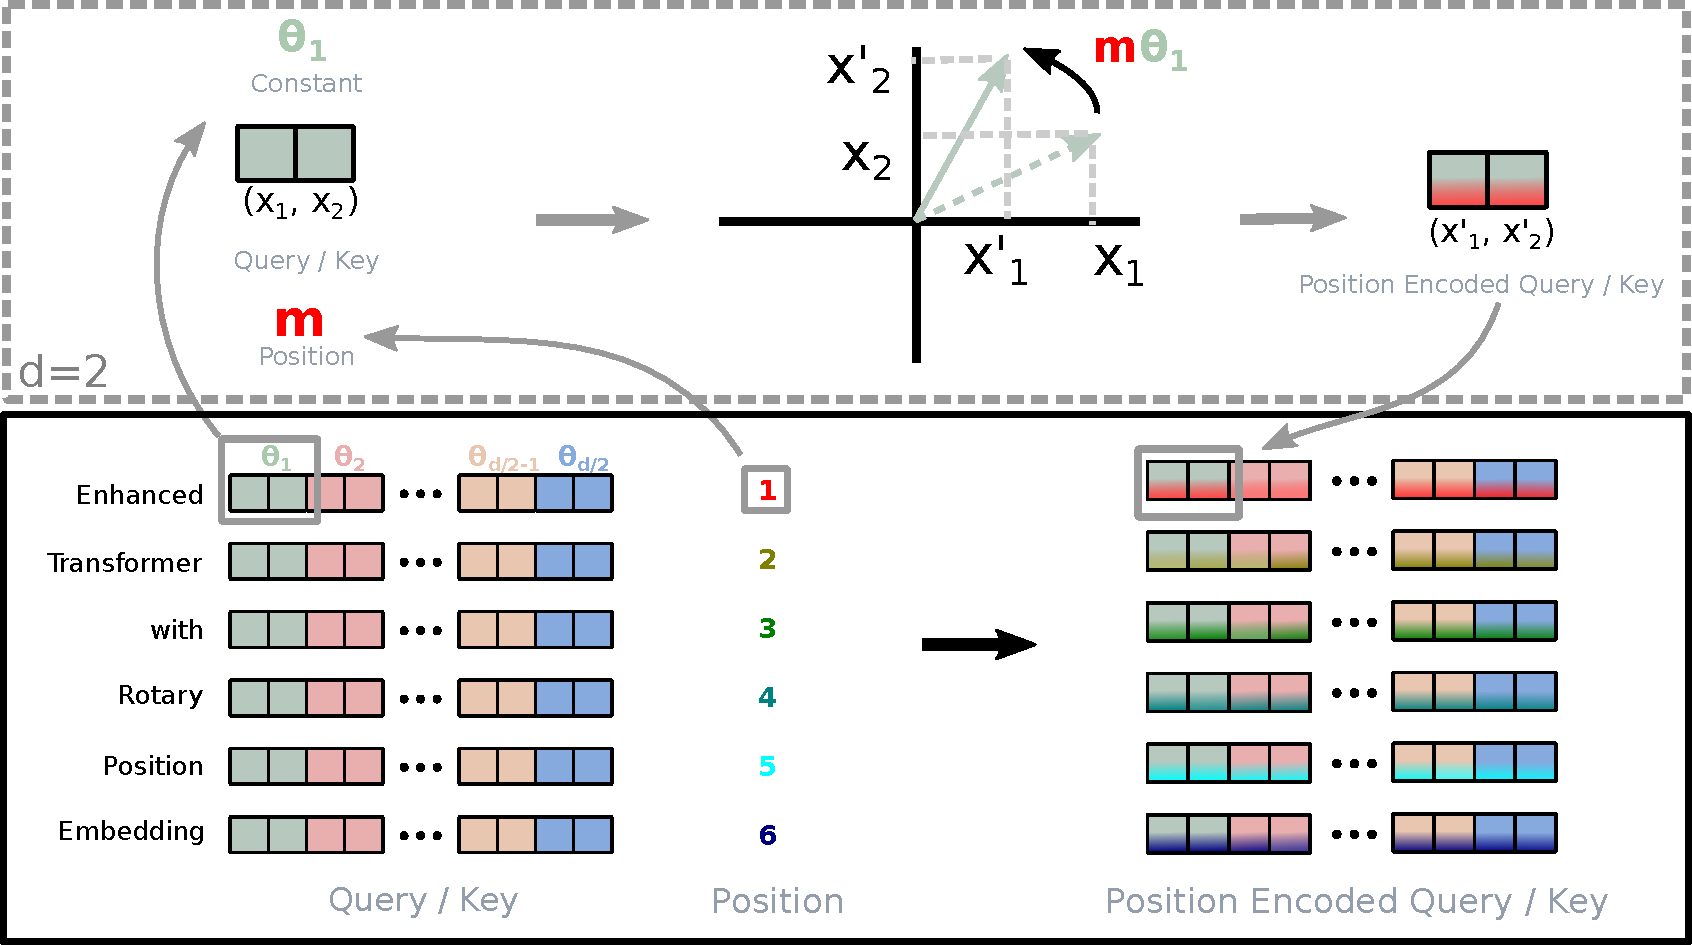
\includegraphics[width=0.9\textwidth]{attachments/RoPE.pdf}
        \\[1ex]
        \textit{Implementation of Rotary Position Embedding (RoPE).}
    \end{center}
\end{frame}

% RoPE: A 2D case
\begin{frame}
    \frametitle{RoPE: A 2D case}

    Let $\x_j$ be from $\mathbb{C} \simeq \mathbb{R}^2$ space, $i = \sqrt{-1}$ and $\theta \in \mathbb{R}$ some frequency. \pause Then RoPE can be formulated as follows


    \begin{equation*}
        \begin{aligned}
    	f_q(\x_m, m) & := (\W_q\x_m)e^{im\theta} \in \mathbb{C},\\
    	f_k(\x_n, n) & := (\W_k\x_n)e^{in\theta} \in \mathbb{C},\\
            f_v(\x_n, n) & := \W_v\x_n,
        \end{aligned}
    \end{equation*}
    which requires extending the query-key inner product by taking only the real part of the number:
    \begin{equation*}
        \langle \q_m \mid \k_n \rangle = \operatorname{Re}[\q_m^{\intercal}\k_n] = \cdots = \operatorname{Re}[(\W_q\x_m)(\W_k\x_n)^{*}e^{i(m - n)\theta}].
    \end{equation*}

    \pause
    The last equation highlights the relative nature of this positional encoding method. 
\end{frame}

% RoPE: General form
\begin{frame}
    \frametitle{RoPE: General form}

    The generalization of the described approach consists of introducing different frequencies in 2D chunks, which can be written as matrix multiplication:

    \begin{equation*}
	f_{\{q, k\}}(\x_m, m) = \R^d_{\Theta, m}\W_{\{q, k\}}\x_m,
    \end{equation*}
    where 
    \begin{equation*}
    \scalebox{0.8}{$
    	\R^d_{\Theta,m} = 
    	\begin{pmatrix}
    		\cos{m\theta_1}& -\sin{m\theta_1}&0&0&\cdots&0&0\\
    		\sin{m\theta_1}&\cos{m\theta_1}&0&0&\cdots&0&0 \\
    		0&0&\cos{m\theta_2}& -\sin{m\theta_2}&\cdots&0&0\\
    		0&0&\sin{m\theta_2}&\cos{m\theta_2}&\cdots&0&0 \\
    		\vdots&\vdots&\vdots&\vdots&\ddots&\vdots&\vdots\\
    		0&0&0&0&\cdots&\cos{m\theta_{d/2}}& -\sin{m\theta_{d/2}}\\
    		0&0&0&0&\cdots&\sin{m\theta_{d/2}}&\cos{m\theta_{d/2}}
    	\end{pmatrix}
    $}
    \end{equation*}
    is the rotary matrix with pre-defined parameters $\Theta = \{\theta_k=10000^{-2(k-1)/d}, k \in \{1, 2, ..., d/2\}\}$.

    \vfill
    The multiplication of this orthogonal sparse matrix by a vector can be implemented in $\mathcal{O}(d)$ time.
\end{frame}

% RoPE: Properties
\begin{frame}
    \frametitle{RoPE: Properties}

    \begin{itemize}
        \item Outperforms aforementioned baselines,
        \item Used in all attention layers, not just the first one,
        \item Do not add any positional noise to the token embedding stream,
        \item Depends only on the relative distance $m - n$ between tokens,
        \item Has strong interpolation and weak extrapolation capabilities.
    \end{itemize}

    \begin{center}
        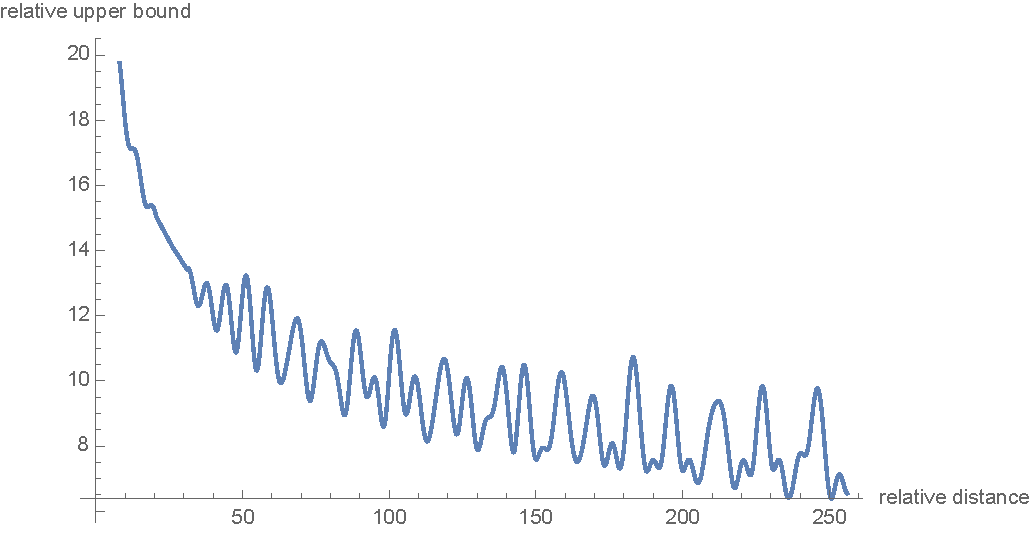
\includegraphics[width=0.5\textwidth]{attachments/long-term-decay.pdf}
        \\[1ex]
        \textit{Long-term decay of the attention scores given \\ \textbf{semantically equal} pair of tokens.}
    \end{center}
\end{frame}

%%
%% HiRoPE
%%
\section[HiRoPE]{HiRoPE}

% HiRoPE: Hierarchical format
\begin{frame}
    \frametitle{HiRoPE: Hierarchical format}

    \begin{columns}
    \column{0.8\textwidth}
    \vbox to .8\textheight{%
    Let $\m = (m_1, \ldots, m_h)^T \in \mathbb{N}_0^h$ represent a vector of positional indices, where $h$ is the number of hierarchical levels.

    \vfill
    Then HiRoPE is applied as follows:
    \vfill
    \begin{enumerate}
        \item Split the initial vector into $h$ chunks, ensuring that each chunk has an even size.
        \item Apply RoPE to each chunk independently, using the corresponding index from $\m$.
        \item Concatenate the result.
    \end{enumerate}
    
    \vfill
    In the experiments, the authors set $h = 2$, which results in $\m = (\textcolor{red}{m_1}, \textcolor{blue}{m_2})^T$, and denote the last dimension of the first chunk as $d_s$.
    \vfill
    When $h = 1$, HiRoPE reduces to RoPE.
    }%
    \column{0.2\textwidth}
    \vbox to .8\textheight{%
    \[
    \begin{pmatrix}
    \textcolor{red}{x_1} \\
    \textcolor{red}{x_2} \\
    \textcolor{red}{\vdots} \\
    \textcolor{red}{x_{d_s}} \\
    \textcolor{blue}{x_{d_s+1}} \\
    \textcolor{blue}{x_{d_s+2}} \\
    \textcolor{blue}{\vdots} \\
    \textcolor{blue}{x_d}
    \end{pmatrix}
    \]
    \vfill
    }%
    \end{columns}
\end{frame}

% HiRoPE: Window mechanism
\begin{frame}
    \frametitle{HiRoPE: Window mechanism}

    \begin{center}
        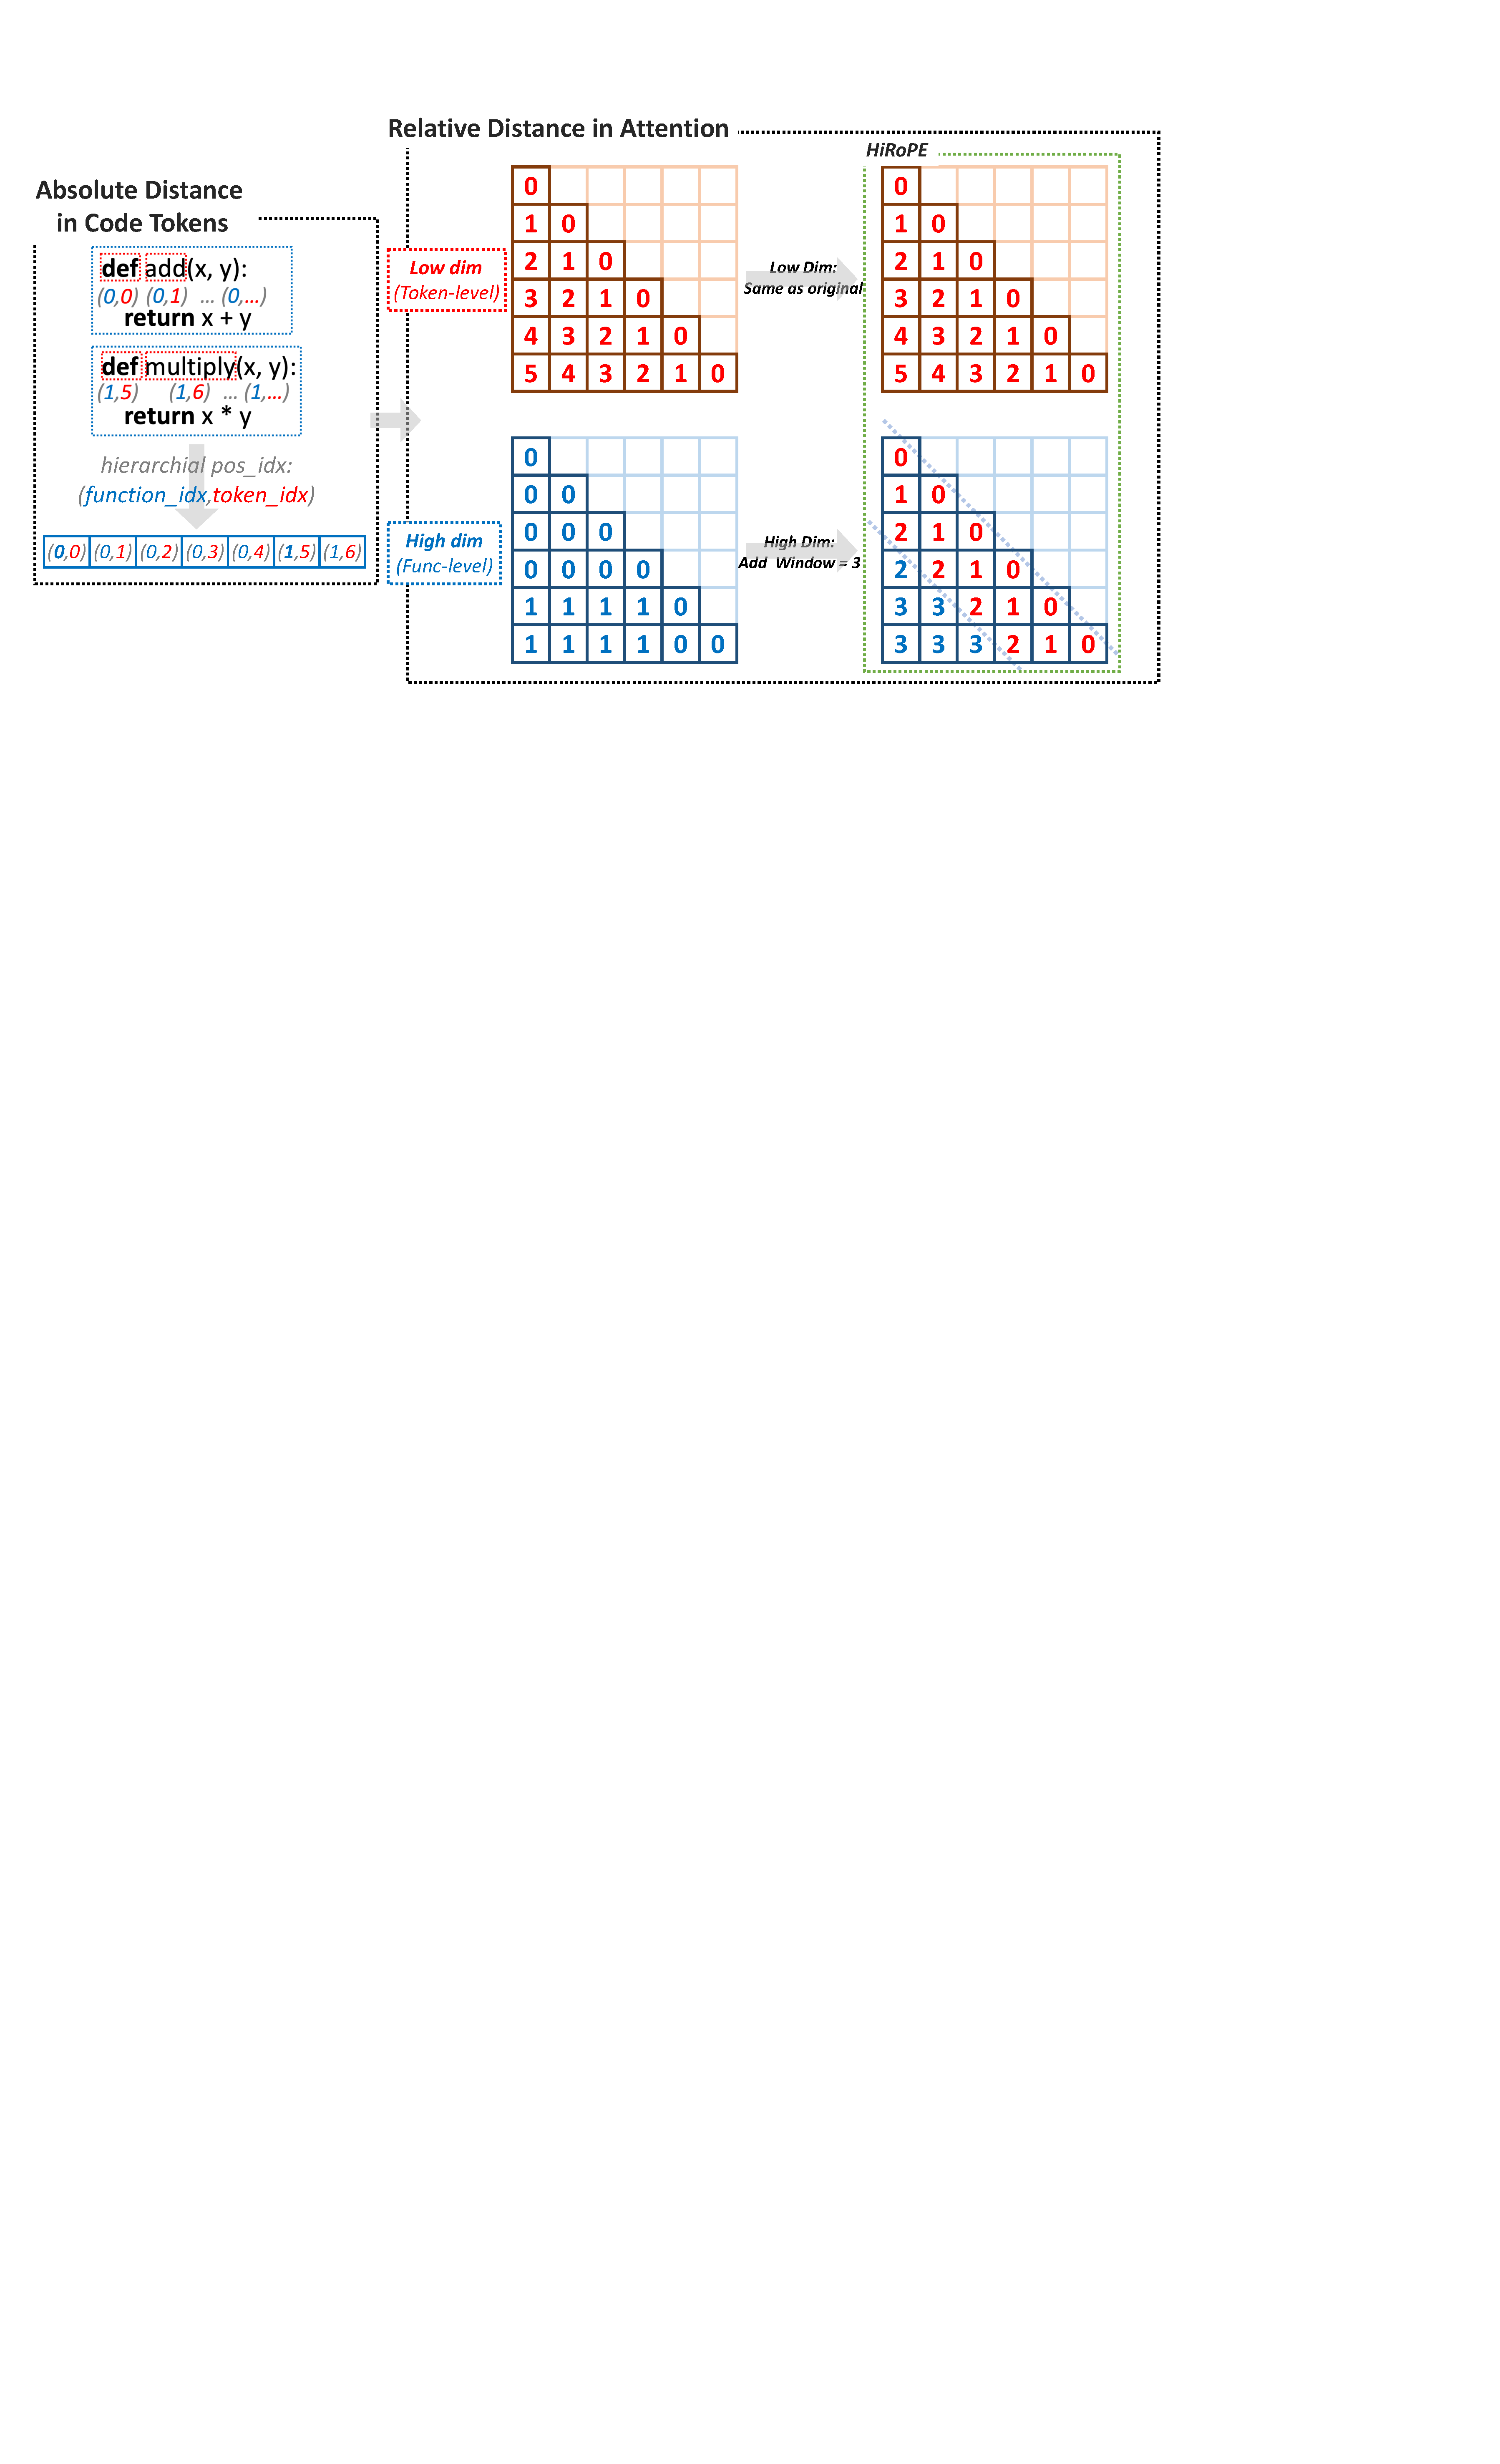
\includegraphics[width=1.0\textwidth]{attachments/window-mechanism.pdf}
        \\[1ex]
        \textit{Positional indices overview} ($L_{window}=3$).
    \end{center}
\end{frame}

% HiRoPE: Results
\begin{frame}
    \frametitle{HiRoPE: Results}

    \begin{center}
        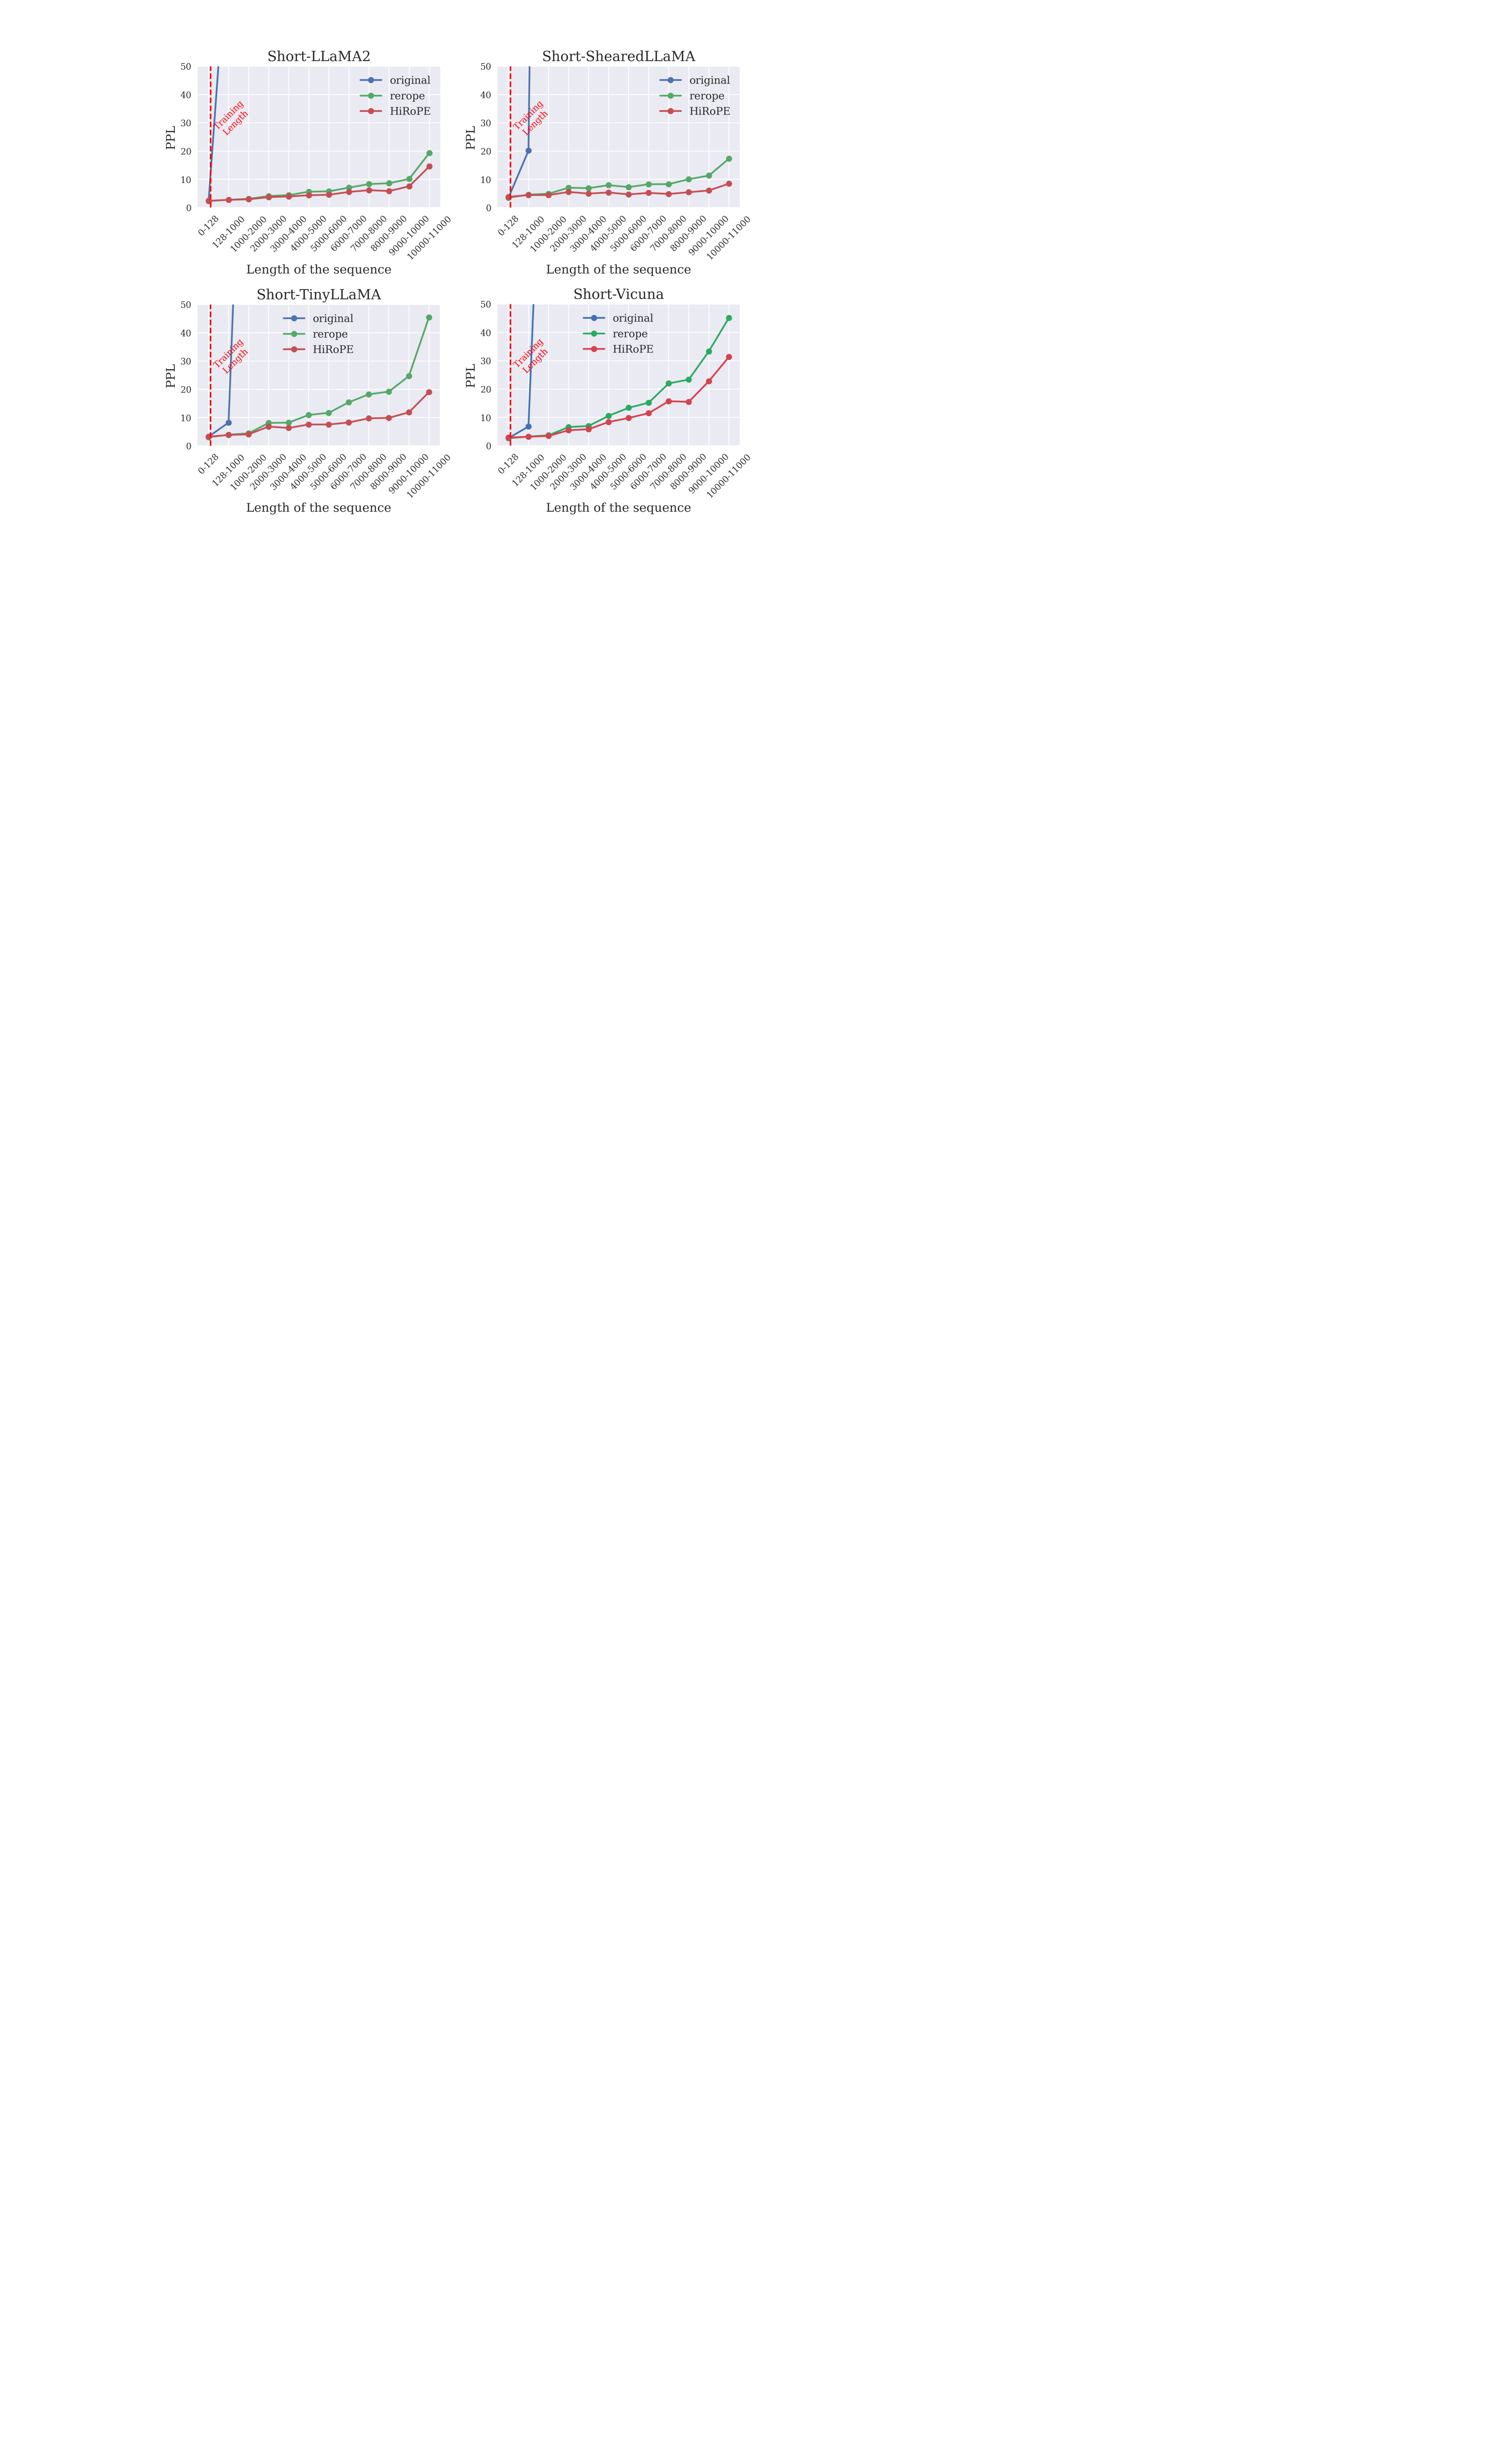
\includegraphics[height=0.75\textheight]{attachments/results.pdf}
        \\[1ex]
        \textit{Performance of ShortLLMs on CodeParrot dataset.\\ The training length is set to 128.}
    \end{center}
\end{frame}

% HiRoPE: Doubts
\begin{frame}
    \frametitle{HiRoPE: Doubts}

    \begin{itemize}
        \item The authors did not provide the code.
        \vfill
        \item The statement about the exponential increase in length does not address the trade-off between the chunk size and the range of indices it can represent.
        \vfill
        \item It is strange that the experiments are strongly limited to $h = 2$.
        \vfill
        \item The window mechanism looks like a quick-and-dirty solution.
        \vfill
        \item There are no experiments verifying whether the hierarchical information is utilized, as opposed to the entire impact coming from clipping RoPE frequencies.
    \end{itemize}
\end{frame}

%%
%% Appendix
%%
\appendix



\end{document}
